\section{Rubin Observatory Commissioning}
\label{sec:commissioning}

\subsection{Commissioning Plan and Schedule}
\label{ssec:commissioning-schedule}

Figure~\ref{fig:commissioning-es-schedule} shows the detailed schedule of commissioning and early science activities relative to Rubin First Light, as of \currentdate.
\begin{figure}[htb]
\centering
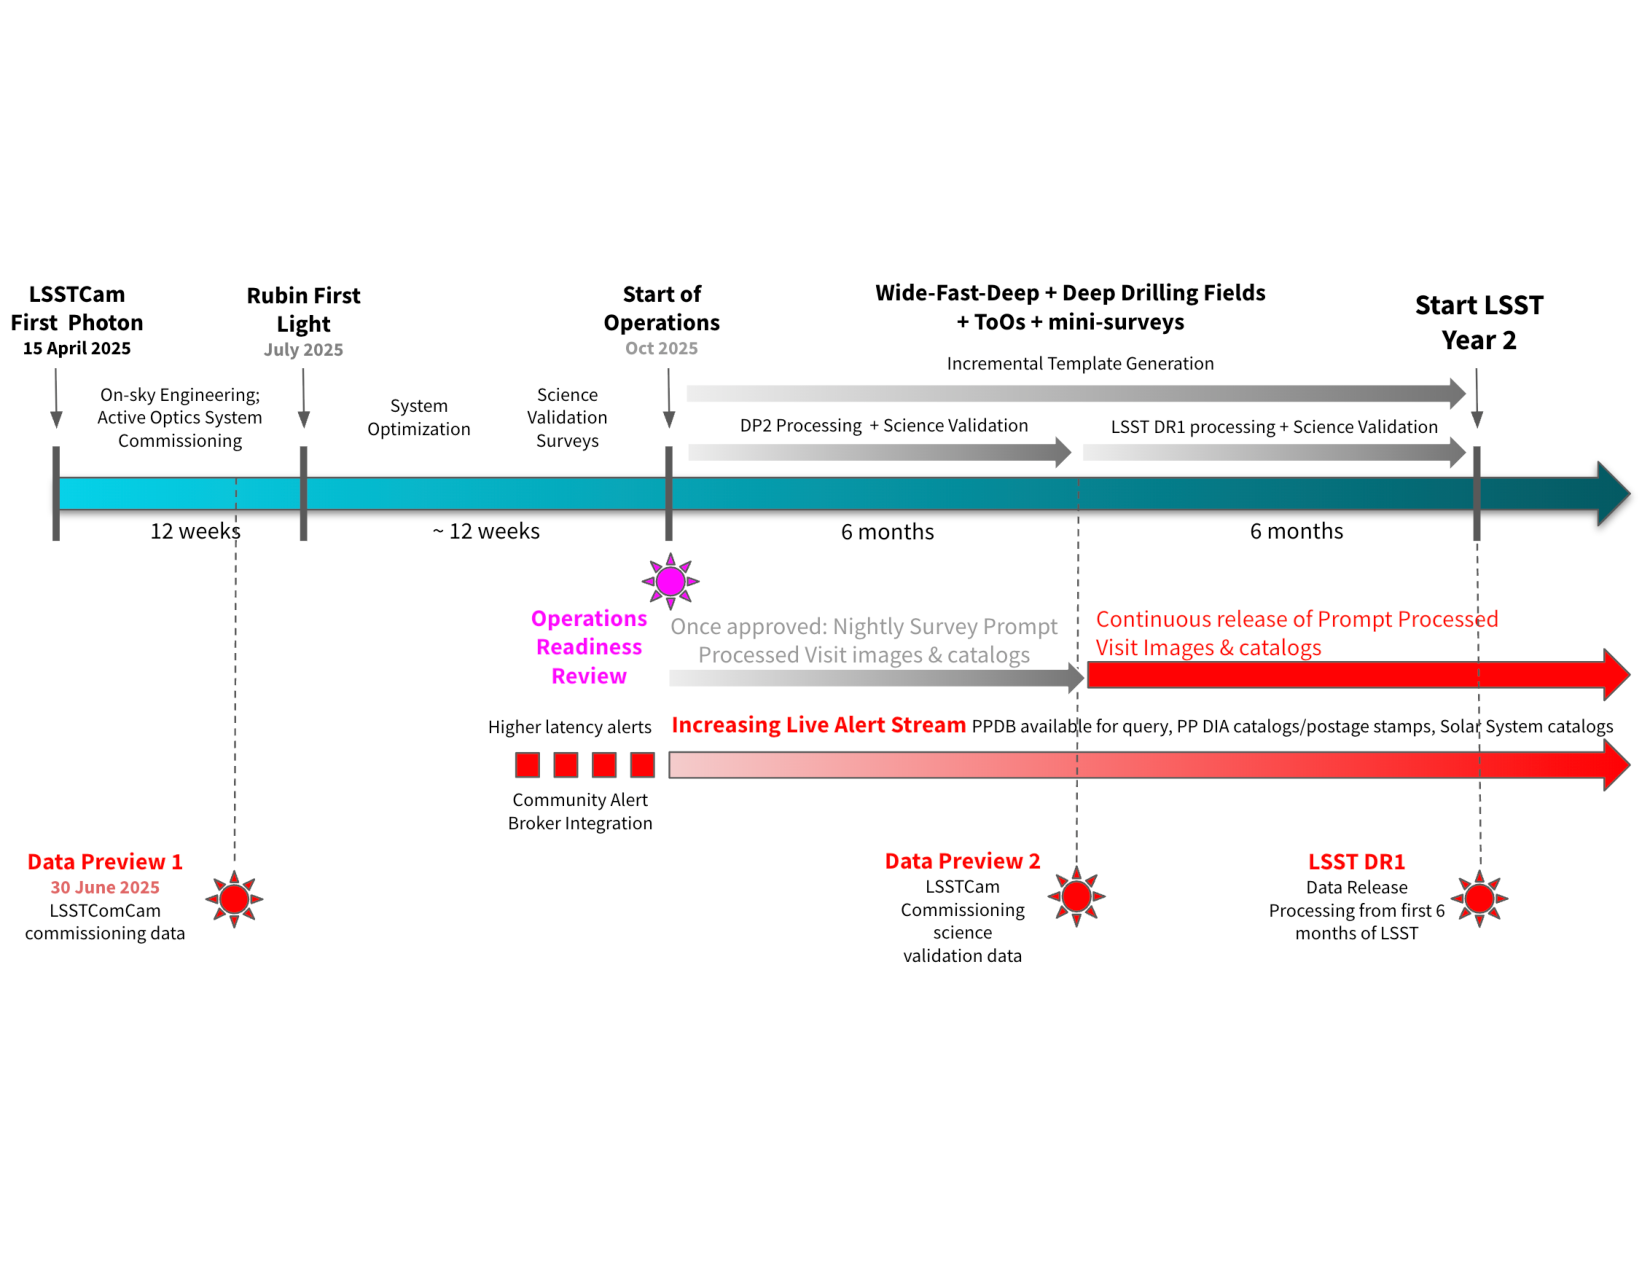
\includegraphics[width=0.98\linewidth]{rubinobs_on-sky_commissioning_and_early_science}
\caption{Detailed schedule of commissioning  and early science activities relative to Rubin First Light, as of \currentdate.}
\label{fig:commissioning-es-schedule}
\vspace{0.1cm}
\end{figure}
LSSTComCam First Photon was successfully achieved on \ccfpdate, followed by Rubin  First Photon with LSSTCam on \lcfpdate.
Rubin First Light is currently expected or \rfldate (\S~\ref{sec:timeline}).

Figure~\ref{fig:commissioning} shows the high level plan for the Rubin commissioning observations.
\begin{figure}[hbt]
\centering
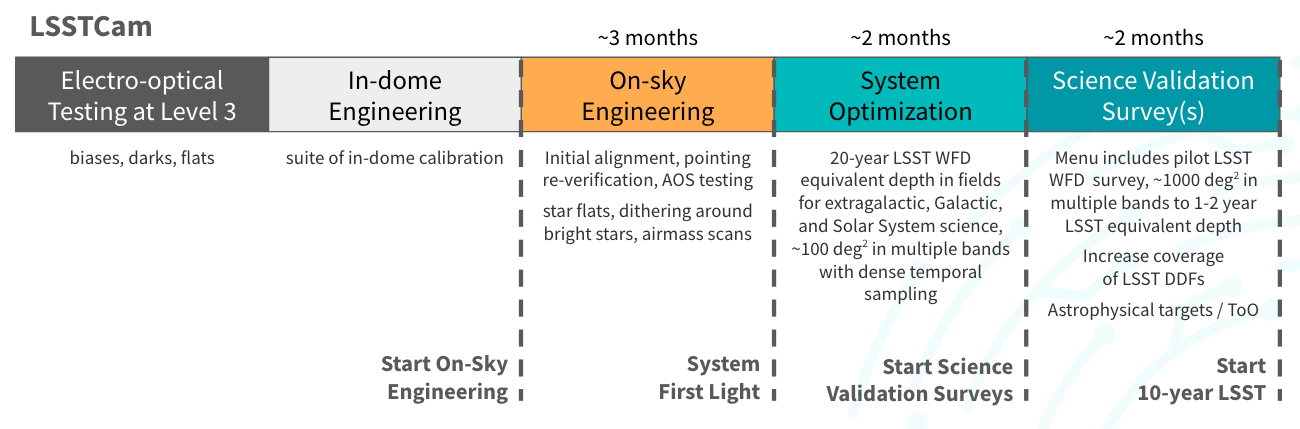
\includegraphics[width=0.95\linewidth]{commissioning-plan}
\caption{Outline plan for the collection of commissioning data, as of \currentdate.}
\label{fig:commissioning}
\end{figure}
Commissioning data collection is planned to take place in phases.
The On-Sky Engineering phase began with LSSTComCam and is continuing with LSSTCam.
Both the System Optimization and Science Validation (SV) phases will be carried out with LSSTCam.
The System Optimization phase will collect a set of observations designed to help optimize the system prior to starting the Science Validation phase.
During the Science Validation phase, a series of SV Surveys designed to support scientific analyses that validate the system's performance and allow Rubin to demonstrate operational readiness will be carried out.
The System Optimization and SV phases contain a number of planned key components, which currently include an LSST wide-fast-deep (WFD) 1--2 year equivalent depth ``pilot'' survey and a
10+~year ``ugrizy'' depth test in three fields covering 100~sq. deg.
In all phases, field selection will be carried out by the commissioning team, taking into account a wide variety of constraints as well as a ``menu'' of science opportunities to which the Rubin Science Community has contributed.
See Section 6 of \citeds{SITCOMTN-005} for the baseline design of the SV surveys.
All plans for commissioning observations are subject to change based on system readiness up until the moment of execution.

The project schedule will continue to evolve as the remaining subcomponents are delivered.
Construction is expected to complete and LSST data taking start before the end of 2025.

\subsection{Key Commissioning Milestones}
\label{ssec:commissioning-milestones}

Commissioning work is being planned around three major milestones, \textit{LSSTComCam First Photon}, \textit{LSSTCam First Photon} and \textit{Rubin First Light}.

\textbf{ComCam First Photon}: The first image of the night sky produced by photons passing through the Rubin optical system and detected by the Commissioning Camera (LSSTComCam).
This milestone was achieved on \ccfpdate.

\textbf{LSSTCam First Photon}: The first image of the night sky produced by photons passing through the Rubin optical system and detected by the LSST Science Camera (LSSTCam).
This milestone was achieved on \lcfpdate.

\textbf{Rubin First Light}: Defined as the point at which we can routinely acquire science-grade imaging across the LSSTCam full focal plane and have a well understood technical path towards meeting the Construction Completeness criteria described in \citeds{sitcomtn-061}.
Currently expected for \rfldate.

LSSTCam First Photon occurs following the successful completion of system integration.
There are no quality criteria applied to achieving the LSSTCam First Photon  milestone.
Rubin First Light  marks the end of the  on-sky engineering phase and the start of the System Optimization and Science Validation phases of commissioning.
The period between LSSTComCam First Photon and Rubin First Light will focus on fine-tuning the system including optical alignment,  improving the image quality, and collecting calibration data.
For a detailed description of all  commissioning milestones and the most current dates, see \citeds{dmtn-232}.

\subsection{LSSTComCam Commissioning}
\label{ssec:commissioning-comcam}

LSSTComCam \citep{10.71929/rubin/2561361} is Rubin's engineering camera that is used for testing and validating the observatory's systems and processes prior to installation of the LSST Camera.
The LSSTComCam focal plane has single raft with a 3×3 mosaic of 4K×4K ITL science sensors, giving a total of 144Mpix,
LSSTComCam has the same plate scale as LSSTCam (0.2 arcsec / pixel), with a field of view of 40 × 40 arcmin.
The LSSTComCam filter exchanger holds only three physical filters at a time.

The Rubin on-sky commissioning campaign using  LSSTComCam began on 24 October 2024 and ended on 11 December 2024, lasting a total of 7 weeks, and included observations to support both engineering and science pipelines commissioning.
This highly successful campaign included a first series of on-sky engineering tests demonstrating the end-to-end functionality of the Simonyi Survey Telescope’s hardware and software systems  LSSTComCam.
The median delivered image quality for commanded in-focus images collected during the campaign, quantified in terms of the PSF FWHM, was $\approx1.1$ arcseconds.
The best images have delivered PSF FWHM of $\approx0.7$ arcseconds.
A full report on the  LSSTComCam on-sky commissioning campaign is available at \citeds{sitcomtn-149}.


\subsection{LSSTCam Commissioning}
\label{ssec:commissioning-lsstcam}

As of \currentdate, LSSTCam \citep{10.71929/rubin/2571927} is installed on  the Simonyi Survey Telescope \citep{2024SPIE13094E..09S} and on-sky commissioning is ongoing.
